\documentclass[12pt]{article}

\usepackage{graphicx}
\usepackage{tabularx}
\usepackage{float} % here for H placement parameter
\usepackage{longtable}

\makeatletter
\setlength{\@fptop}{0pt}
\makeatother


\title{Experimental Method - Planning}
\author{
\\
  Louis Cameron Booth\\
  \texttt{louiscb@kth.se}
  \and
  \\
  Matay Mayrany\\
  \texttt{mayrany@kth.se}
  \\
  \\
}
\date{\today}

\begin{document}
\maketitle

\begin{center}

\includegraphics[width=3cm]{logo.png}
\end{center}

\pagebreak
\tableofcontents
\newpage
\section{Impact Goals and Objectives}

 The goal of and the motivation behind the experiment is to provide a detailed image of the benefits and shortcomings of two different implementations of the priority queue. This will be considered based on the which of two use-cases they are targeting. The first of the two implementations being evaluated is based on the data structure of a singly linked list, while the second is based on the heap. 
Each of these data structures will be used to make priority queues for the following use-cases (see Figure 1): 

\begin{itemize}
   \item Future pending event sets in event-driven simulations: what events this will be developed for is abstract and depends on the developer, as it can be any case where scheduling of events based on priority is the aim. The priority here is represented using timestamp doubles, where the one with the nearest stamp should be dequeued first.
   \item Ready queue for processes and threads in operating systems:
 this refers to the scheduling of processes where the CPU needs to decide for which one it should allocate resources. The priority here is represented using a discrete set of integers where the one with the highest value should be dequeued first. \end{itemize}

The value behind priority queues and general scheduling concepts for both, or in fact any use case is well described by the following quote from 3 Easy Pieces by Remzi and Andrea Arpaci-Dusseau:
\\
\\
 \textit{“The origins of scheduling, in fact, predate computer systems; early approaches were taken from the field of operations management and applied to computers. This reality should be no surprise: assembly lines and many other human endeavours also require scheduling, and many of the same concerns exist therein, including a laser-like desire for efficiency” [6].} \\

Hence, this report and the results of these experiments can be used by someone who wished to capture the value described above by building an application that is relevant to the context of the experiment. That is, if they wish to use a priority queue in their application and they need to decide on an implementation based on the context, they can refer to such experiments or carry out a variation of their own. 

This will hopefully also benefit the users of the developed application as it gives them the best possible implementation for the intended use case. The best implementation should provide the best access time for the elements in the system, and thus a smoother experience for a user of the application.

 A deeper look into this experiment and the results in specific contexts will help us understand and make decisions on when the implementations are relevant. 

\section{Preliminary study}

We can analyse the different queues based on the theory and the expected performance of the data structures. We can also consider what factors and variables will affect this performance and predict their effects. In order to do this we need to take a look at what happens in each use case. 

 The specifications and testing choices for the event-driven simulations implementation are the following: 

\begin{itemize}
   \item The priorities are represented using timestamps that function as explained previously. 
   \item After every dequeue of an element 0-N new elements are generated using the dequeued element’s timestamp added to a randomly generated increment() value. For simplicity, we will generate 2 events for each dequeue. 
   \item The simulation will end when a limit of events (elements) is reached in the queue (L).
   \item If two events have identical timestamps we should use FIFO and dequeue the one that was added first. 
\end{itemize}

As a result we will need to consider this entire process every time we access the queue in our study in order to find out how effective the data structures are for this specific situation. We need to judge the two data structures for the operation of removing() the highest priority element and inserting() 2 with a random priority. 
\\
\\
The specifications and choices we made for the use case of a ready queue are the following: 

\begin{itemize}
   \item The priority is represented using integer values in a predefined discrete set. 
   \item The testing will be done by making N number of enqueues followed by the same number of dequeues. Chosen based on Up/Down model proposed by Rönngren  \cite{robert}. 
\end{itemize}

We will also need to keep these in consideration when testing and comparing the two implementations.

\subsection{Variables} 
\textbf{Independent Variables}  - \textit{Variables we choose and alter to see the effect on the dependent variables and the performance.}
\begin{itemize}
 \item The limit for queue size in event-driven simulations (L). Different numbers should be tested to see what implementation is good for what size. Specified by us in the testing program.
\item The number of enqueues followed by the same number of Deques (N). Similarly multiple values should be used with both implementations. Specified by us in the testing program.
\end{itemize}
\textbf{Dependent Variables} - \textit{Variables that we Measure in order to evaluate performance of the implementations.}
\begin{itemize}
\item Execution Time. Used to determine performance of both data structure and measured using the clock() function in C. The implementation that provides the lowest access time and returns the value in the lowest execution time would prove superior.
\end{itemize}
\textbf{Control Variables}- \textit{Variables that we need to keep constant throughout the experiment to collect fair data.}
\begin{itemize}
\item The hardware we are using to carry out testing. Different hardware and processing speed can lead to different execution time results. The specifications of the hardware used can be seen in section 5 of this report. 
\end{itemize}
The experiment over all can be described by \textit{Figure 1}, where we will implement four versions of the priority queue based on the two data structures. We will then test the implementations based on the use case. This will be done by controlling and varying the relevant variables in the experiment when testing for the context. 

\begin{center}
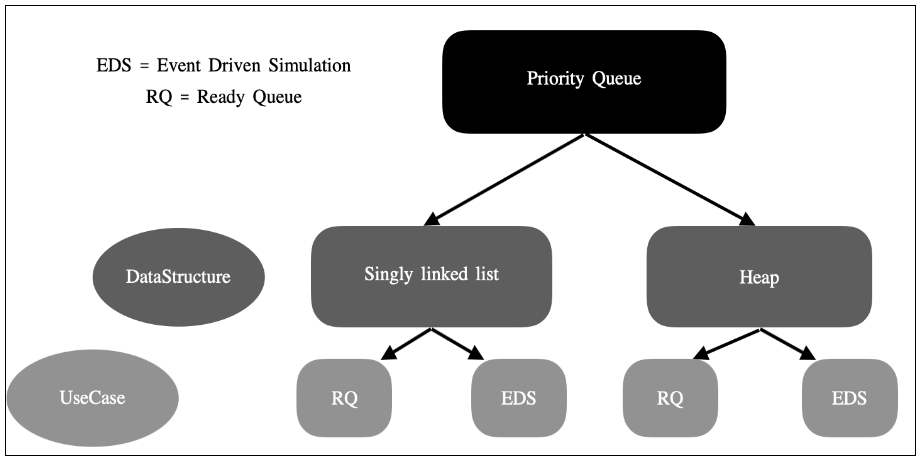
\includegraphics[width=15cm]{figure-1.png}
\end{center}

\section{Methodology}

 The study will mostly be using quantitative and inductive methods as we will be carrying out experiments and observing the results to draw conclusions. The observed results are those of numerical value (Execution Time). This is also true for the independent variables of the experiment, as the performance is expected to be affected by altering the numeric value of these variables, which brings up the quantitative aspect of the experimentation. Some qualitative input will also be included if we come across it throughout the process. An example could be an input on the ease of implementation of the priority queues, using the two data structures in the different scenarios. Keeping in mind any potential tradeoff it might have on performance. 
 
\section{Experiment plan}

We will make two sets of experiments where we compare the priority queues in different contexts. We will measure the behaviour of single linked lists and heap based priority queues using random priorities with a high entropy. The reason we will use random priorities is to provide an accurate environment for experimentation. According to the department of Statistics \& Data Science of Yale “it is generally extremely difficult for experimenters to eliminate bias using only their expert judgment, therefore the use of randomisation in experiments is common practice” [2]. 
\\
\\
For the experiment testing of the ready queues we will follow the Up/Down model proposed by Rönngren, where “a sequence of enqueues is followed by an equally long series of deques” [1], in order to measure performance. 
\\
\\
For the experiment testing of the event driven queues we will take a different approach where we will simulate an event driven environment. For each event dequeued from queue, we will enqueue two elements where the priority is a timestamp with an added random value.
\\
\\
In our measurement of performance we will analyse both the average access time and the worst case performance of each implementation. In order to generate accurate measurements, we will run our experiments for an allocated duration of time before taking measurements in order to prevent our data being corrupted by extreme data points [1]. Our data collection will measure each individual enqueue \& dequeue operation in order to “isolate the effects of the underlying hardware”, we will also preallocate the necessary memory for the programs before running the experiments to minimize the underlying effects of the memory management system [1]. 


Our code implementing the algorithms will be written entirely in the programming language C. Other more modern languages usually contain overheads which could impact the accuracy of our measurements, such as garbage collection. Elements in the queue will be organised by priority and when multiple elements have the same priority then they will be arranged in a First In First Out (FIFO) order.

\subsection{Time measurement of queue operations}

As our algorithms will be implemented in C, our measurements of these algorithms will also be implemented in C. We will use the function clock() that is available in the time.h package. As mentioned previously, we will measure individual enqueue and dequeue operations. We will store the value of the clock() function prior to the beginning of the queue process we are measuring, and then at the end after the operation has successfully been executed. We will find the difference between the clock values before and after our operation and then divide it by the number of ticks per second for our CPU.  This will give us a measurement of our operation in the SI base unit of second.
\\
\\
It is also important to note that the clock() operation itself takes a certain amount of time to run which will inaccurately be included in our recorded results. To counteract this we will obtain the amount of time clock()  takes to run with no operations and subtract this value from the recorded time of the queue operations. To maintain accuracy, the hardware with which we make our measurements will have to remain consistent, we expand on this in section 5 of this document. 
\\
\\
With this measurement technique we will obtain average and worst case times for our algorithms. We will determine the average time complexity of each implementation by calculating the mean of the time of the recorded operations. We will determine the worst case by taking the highest value of time of each implementation.

In table 1 we have the big O time complexities of our algorithms and will be using these as a point of reference throughout the experiment.    

\begin{table}[h]
\caption{ Time Complexities of Algorithms [3]}
\begin{tabular}{|l|l|l|ll}
\cline{1-3}
\textbf{Algorithm}                & \textbf{Average Case} & \textbf{Worst Case} &  &  \\ \cline{1-3}Heap Based - Event                & O(log(n))    & O(log(n))  &  &  \\ \cline{1-3}
Heap Based - Ready Queues         & O(log(n))    & O(log(n))  &  &  \\ \cline{1-3}
Singly Linked List - Event        & O(n)         & O(n)       &  &  \\ \cline{1-3}
Singly Linked List - Ready Queues & O(n)         & O(n)       &  &  \\ \cline{1-3}
\end{tabular}
\end{table}

\subsection{Random generation}

As mentioned previously, we will be randomly generating priority for the elements that we add to our queues. We will therefore need a method of generating a sequence of pseudorandom numbers in C. According to the Software Engineering Institute of Carnegie Mellon University “The C Standard rand() function makes no guarantees as to the quality of the random sequence produced” [4]. As a result we will use OpenBSD’s arc4random family of funct are cryptosecure and appear with distributions of OpenBSD, Darwin and Linux. According to OpenBSD’s manuals arc4random “provides higher quality data than those described in rand, random and rand48” [5]. 

\section{Experimental setup}

In order to reduce the impact of hardware, we will consistently use the same machine for all our testing. Below are the hardware specifications of the computer.

\begin{verbatim}
Macbook Pro, 13-inch, Early 2015
Processor 2,7 GHz Intel core i5
Memory 8 GB 1867 MHz DDR3
Operating System macOS Mojave 10.14.1
\end{verbatim}

In the same vain, we will use the same C compiler and version for all running of the experiments. Below are the compiler specifications.

\begin{verbatim}
GCC
Version 9.0.0
Thread Model: Posix
\end{verbatim}

In order to remove human error and bias from our measurements, we will automate as much of the experimental process as possible. To do this we will create a bash script that will run our compiled programs and output the values of  these programs into a CSV file for us to analyse. Automating our experimental process as a bash script will allow us to collect large volumes of data very quickly and will give us a fixed testing environment where we can alter certain parameters. Our bash script will test our algorithms using a range of different queue sizes. We have predefined these values.

\begin{verbatim}
Queue Sizes - 5, 10, 20, 50, 100, 200, 500, 1000, 2000, 5000
\end{verbatim}

The reason for having such a large range of queue sizes is because we predict the different algorithms to perform very differently depending on the size of the set of the data it has to process. According to Douglas W. Jones “priority queues are the best for fewer than 10 items, although they perform very poorly for queues of more than 50 items” [7]. This will give us a better understanding of which implementation to use depending on the context.
\\
\\
As illustrated in figure 1, we will be testing four separate implementations and we will run each implementation through the range of queue sizes 100 times in order to collect a large enough set of data to draw conclusions from. 

An overview of our program set up is as follows:  four separate C programs for each queue implementation, main C program that calls and times queue implementations, testing bash program.

In order to validate our experimental setup we will use unit testing to check the individual modules and functions that make up our program. Unit testing will allow us to continually check the performance of our code as we build our experiment. We have chosen cUnit as our unit testing library since it is a lightweight framework that is user friendly [8].


\section{When have the goals identified been met? When are the experiments done?}

The goals \& experiments are complete once we have gathered data of an acceptable quality and size with which we can determine conclusions about the performance of the implementation of priority queues. We aim for this experiment to provide enough information for us to propose valid hypotheses on the use of priority queues in different contexts, and compare their use to each other.

\section{Requirements table}

\begin{table}[H]
\caption{Table of requirements for project}
\label{BT2}
\footnotesize
% \resizebox{\textwidth}{!}{%
\begin{tabular}{|p{1cm}*{4}{|p{\dimexpr(\textwidth-1cm)/4\relax}}|}%{|l|l|l|l|l|}
\hline
\textbf{Req. \#} & \textbf{Type of Requirement} & \textbf{Designation Source} & \textbf{Description of the requirement} & \textbf{Completed / Not met / Partially met} \\ \hline
1 & Must Have & Implement Priority Queue based on Single-Linked List Event Driven & Implement a priority queue for Event Driven use cases, in C, using the single linked list data structure. & NC \\ \hline
2 & Must Have & Implement Priority Queue based on Single-Linked List Ready Queue & Implement a priority queue to fit the criteria of a ready queue in C, using the single linked list data structure. & NC \\ \hline
3 & Must Have & Implement Priority Queue based on Heap Event Driven & Implement a priority queue for Event Driven use cases, in C, using the heap data structure. & NC \\ \hline
4 & Must Have & Implement Priority Queue based on Heap Ready Queue & Implement a priority queue to fit the criteria of a ready queue in C, using the heap data structure. & NC \\ \hline
5 & Should Have & Create unit testing for our implementation of our programs & Use cUnit to create unit testing for the many functions in all our code for our programs. & NC \\ \hline
6 & Should Have & Implement automated queue testing program & Create a bash program that automates the testing process of our queues. & NC \\ \hline

\end{tabular}%
% }
\end{table}

\begin{table}[H]
\label{BT2}
\footnotesize
% \resizebox{\textwidth}{!}{%
\begin{tabular}{|p{1cm}*{4}{|p{\dimexpr(\textwidth-1cm)/4\relax}}|}%{|l|l|l|l|l|}
\hline

\textbf{Req. \#} & \textbf{Type of Requirement} & \textbf{Designation Source} & \textbf{Description of the requirement} & \textbf{Completed / Not met / Partially met} \\ \hline
7 & Must Have & Evaluate best, normal, worst case performances for Priority Queue based on Single-Linked List Event Driven & Do an analytical and execution evaluation of the best case, worst case and expected case for the single-linked list priority que. For the Event Driven Simulation use case. & NC \\ \hline
8 & Must Have & Evaluate best, normal, worse case performances for Priority Queue based on Single-Linked List Ready Queue & Do an analytical and execution evaluation of the best case, worst case and expected case for the single-linked list priority que. For the Event Ready Queue use case. & NC \\ \hline
9 & Must Have & Evaluate normal, worst case performances for Priority Queue based on Heap Event Driven & Do an analytical and execution evaluation of the best case, worst case and expected case for the heap priority queue. For the Event Driven Simulation use case. & NC \\ \hline
10 & Must Have & Evaluate normal, worst case performances for Priority Queue based on Heap Ready Queue & Do an analytical and execution evaluation of the best case, worst case and expected case for the single-linked list priority que. For the Event Ready Queue use case. & NC \\ \hline
11 & Must Have & Make Code Available on LINUX servers & Do an analytical and execution evaluation of the best case, worst case and expected case for the single-linked list priority queue. & NC \\ \hline
\end{tabular}%
% }
\end{table}

\begin{thebibliography}{999}
\bibitem{robert}
	\emph{Robert Rönngren and Rassul Ayani},
	A Comparative Study of Parallel and Sequential Priority Queue Algorithms, Royal Institute of Technology
\bibitem{yale}
	\emph{Department of Stats \& Data Science},
	Experimentation, Yale University
\bibitem{algorithms}
	\emph{Robert Sedgewick},
	Algorithms \& Data Structures, Princeton University
\bibitem{carnegie}
	\emph{Software Engineering Institute},
	Confluence, Carnegie Mellon University
\bibitem{openbsd}
	\emph{OpenBSD},
	arc4random Library Functions Manual
\bibitem{operating}
	\emph{Remzi H. Arpaci-Dusseau and Andrea C. Arpaci-Dusseau },
	Operating Systems: Three Easy Pieces
\bibitem{brown}
	\emph{R. Brown},
Calendar queues: a fast priority queue implementation for the simulation event set problem, Communications of the ACM
\bibitem{cunit}
	\emph{CUnit Progammers Guide},
Introduction to Unit Testing with CUnit
\end{thebibliography}

\end{document}
This is never printed
